\addcontentsline{toc}{chapter}{Занятие 17. Центральная предельная теорема}
\chapter*{Занятие 17. Центральная предельная теорема}

\addcontentsline{toc}{section}{Контрольные вопросы и задания}
\section*{Контрольные вопросы и задания}

\subsubsection*{Сформулируйте центральную предельную теорему,
                запишите центральную предельную теорему для последовательности испытаний Бернулли.}

Центральная предельная теорема.
$ \xi_1, \dotsc, \xi_n$ -- независимые одинаково распределённые случайные величины,
$M \xi_1 = a, \,
  D \xi_1 = \sigma^2 < \infty $.
Тогда
$$ \frac{S_n - MS_n}{ \sqrt{D \xi_1}} \overset{d}{ \rightarrow } N \left( 0, 1 \right), \,
  n \to \infty,$$
где
$$S_n =
  \sum \limits_{i = 1}^n \xi_i.$$

Подставляя значения математического ожидания и дисперсии получим
$$ \frac{S_n - na}{ \sqrt{n}} \overset{d}{ \rightarrow } N \left( 0, \sigma^2 \right), \
  n \to \infty.$$

Пусть $ \left\{ \varepsilon_k \right\} $ ---
последовательность независимых одинаково распределённых случайных величин, таких, что
$$ \varepsilon_k =
  \begin{cases}
    1, \qquad p, \\
    0, \qquad 1 - p.
  \end{cases}$$
Тогда
$$ \frac{S_n - np}{ \sqrt{n}} \overset{d}{ \rightarrow }
  N \left( 0, p \left( 1 - p \right) \right).$$

Перенесём $p \left( 1 - p \right)$ влево
$$ \frac{S_n - np}{ \sqrt{n} \sqrt{p \left( 1 - p \right) }} \overset{d}{ \rightarrow }
  N \left( 0, 1 \right).$$

\addcontentsline{toc}{section}{Аудиторные задачи}
\section*{Аудиторные задачи}

\subsubsection*{17.3}

\textit{Задание.} Пусть $ \xi $ --- случайная величина со стандартным нормальным распределением.
Пользуясь таблицей стандартного нормального распределения найдите:
\begin{enumerate}[label=\alph*)]
\item вероятность $P \left( \xi \leq 2.2 \right) $;
\item такое $x$, что $P \left( \xi > x \right) = 0.9$.
\end{enumerate}

\textit{Решение.} $ \xi \sim N \left( 0 ,1 \right) $.
Найдём вероятности
\begin{enumerate}[label=\alph*)]
\item $P \left( \xi \leq 2.2 \right) =
        1 -P \left( \xi > 2.2 \right) =
        1 - \Phi_t \left( 2.2 \right) =
        1 - 0.014 =
        -.986$;
\item изобразим ситуацию на рисунке \ref{fig:173}.

\begin{figure}[h!]
  \centering
  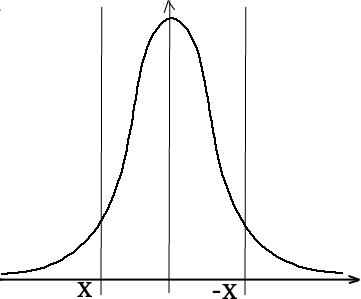
\includegraphics[width=.4\textwidth]{./pictures/17_3.png}
  \caption{Площадь под гаусианой}
  \label{fig:173}
\end{figure}

Площадь каждой половины под графиком равна $0.5$.
Отсюда следует, что $x < 0$.

Получаем, что $ \Phi_t \left( -x \right) = 0.1$.

Ещём в таблице значений $-x = 1.18$.
Значит, $x = -1.18$.
\end{enumerate}

\subsubsection*{17.4}

\textit{Задание.}
Пусть $S_{100}$ --- число гербов, которые выпали при 100 подбрасываниях правильной монеты.
С помощью центральной предельной теоремы приближённо вычислите вероятности:
$$P \left( S_{100} < 45 \right), \,
  P \left( 45 < S_{100} < 55 \right), \,
  P \left( S_{100} > 63 \right).$$

\textit{Решение.} Пусть $ \xi_i = \mathbbm{1}$ \{при $i$-м подбрасывании выпал герб\}.
Тогда
$$S_{100} =
  \sum \limits_{i = 1}^{100} \xi_i.$$

Математическое ожидание введённой случайной величины совпадает с вероятностью того, что выпал герб
$$M \xi_i =
 \frac{1}{2}.$$

Дисперсия равна
$$D \xi_i =
  \frac{1}{2} \cdot \frac{1}{2} =
  \frac{1}{4}.$$

Для суммы
$$MS_{100} = 100 \cdot \frac{1}{2} = 50, \,
  DS_{100} = \frac{100}{4} = 25.$$

Найдём первую вероятность
$$P \left( S_{100} < 45 \right) =
  P \left(
      \frac{S_{100} - MS_{100}}{ \sqrt{DS_{100}}} < \frac{45 - MS_{100}}{ \sqrt{DS_{100}}}
    \right).$$
Первая дробь в скобрах примерно равна случайной величине
$$ \eta \to
  N \left( 0, 1 \right)$$
по центральной предельной теореме
$$P \left( S_{100} < 45 \right) =
  P \left( \eta < \frac{45 - 50}{ \sqrt{25}} \right) =
  P \left( \eta < -1 \right) =
  P \left( \eta > 1 \right) =
  0.159.$$

Следующая вероятность равна
$$P \left( 45 < S_{100} < 55 \right) =
  P \left( -1 < \eta < 1 \right) =
  1 - \Phi_t \left( 1 \right) =
  1 - 2 \cdot 0.159 =
  0.682.$$

Последняя верноятность из таблицы равна
$$P \left( S_{100} > 63 \right) =
  P \left( \eta > \frac{13}{5} \right) =
  P \left( \eta > 2.6 \right) =
  0.005.$$

\subsubsection*{17.5}

\textit{Задание.}
Пусть $ \left\{ \xi_n \right\}_{n \geq 1}$ ---
последовательность независимых одинаково распределённых
случайных величин с распределением Бернулли с параметром
$$p =
  \frac{1}{2},$$
и пусть $S_k = \xi_1 + \dotsc + \xi_k$.
Найдите такое $k$, чтобы
$$P \left( \left| S_k - kp \right| > 1000 \right) >
  0.0455.$$

\textit{Решение.} Математическое ожидание суммы $S_k$ равно
$$MS_K =
  kp =
  k \cdot \frac{1}{2}.$$

Дисперсия равна
$$DS_k =
  k \cdot \frac{1}{4}.$$

Записываем вероятность в таком виде, чтобы можно было применить центральную предельную теорему
$$P \left( \left| S_k - \frac{k}{2} \right| > 1000 \right) =
  P \left(
      \left| \frac{S_k - \frac{k}{2}}{ \sqrt{ \frac{k}{4}}} \right| > \frac{2000}{ \sqrt{k}}
    \right) \approx
  P \left( \left| \eta \right| > \frac{2000}{ \sqrt{k}} \right) >
  0.0455,$$
так как
$$ \frac{S_k - \frac{k}{2}}{ \sqrt{ \frac{k}{4}}} \approx
  \eta \sim
  N \left( 0, 1 \right).$$

Нарисуем график (рис. \ref{fig:175}), закрасим площадь, котороя соответствует тому, что
$$ \left| \eta \right| =
  \left| x \right| >
  \frac{1000}{ \sqrt{k}}.$$

\begin{figure}[h!]
  \centering
  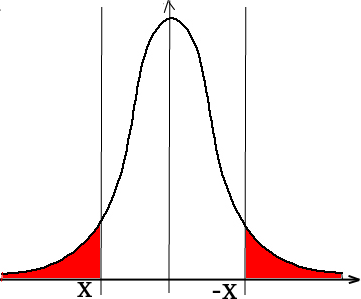
\includegraphics[width=.4\textwidth]{./pictures/17_5.png}
  \caption{Площадь под гаусианой}
  \label{fig:175}
\end{figure}

Тогда
$$2 \Phi_t \left( \frac{2000}{ \sqrt{k}} \right) >
  0.0455.$$

Тогда табличное
$$ \Phi_t \left( \frac{2000}{ \sqrt{k}} \right) >
  0.0275.$$

В таблице значений ищем $0.0275 \approx 0.028$.
Получается
$$ \frac{2000}{ \sqrt{k}} <
  1.91.$$

Отсюда
$$ \sqrt{k} >
  \frac{2000}{1.91} \approx
  \frac{2000}{2} =
  1000.$$
Тогда $k > 10000000$.

\addcontentsline{toc}{section}{Домашнее задание}
\section*{Домашнее задание}
